\documentclass[letterpaper,journal]{IEEEtran}
\usepackage{amsmath,amsfonts}
\usepackage{array}
\usepackage[caption=false,font=footnotesize]{subfig}
\usepackage{textcomp}
\usepackage{stfloats}
\usepackage{url}
\usepackage{verbatim}
\usepackage{graphicx}
\usepackage{booktabs}
\usepackage{cite}
\usepackage{amssymb}
\usepackage{amsthm}
\usepackage{tabularx}
\usepackage{tikz}
\usetikzlibrary{arrows.meta}
\newcolumntype{Y}{>{\centering\arraybackslash}X}

\newtheorem{theorem}{Theorem}
\newtheorem{lemma}{Lemma}
\newtheorem{corollary}{Corollary}
\newtheorem{proposition}{Proposition}
\theoremstyle{definition}
\newtheorem{definition}{Definition}
\theoremstyle{remark}
\newtheorem{remark}{Remark}
\theoremstyle{plain}
\hyphenation{op-tical net-works semi-conduc-tor IEEE-Xplore}
% updated with editorial comments 8/9/2021

\begin{document}

\title{XXXX}

\author{

}
% <-this % stops a space
% \thanks{This paper was produced by the IEEE Publication Technology Group. They are in Piscataway, NJ.}% <-this % stops a space
% \thanks{Manuscript received April 19, 2021; revised August 16, 2021.}}

% The paper headers
% \markboth{Journal of \LaTeX\ Class Files,~Vol.~14, No.~8, August~2021}%
% {Shell \MakeLowercase{\textit{et al.}}: A Sample Article Using IEEEtran.cls for IEEE Journals}

% \IEEEpubid{0000--0000/00\$00.00~\copyright~2021 IEEE}
% Remember, if you use this you must call \IEEEpubidadjcol in the second
% column for its text to clear the IEEEpubid mark.

\maketitle

\begin{abstract}
aaa
\end{abstract}

\begin{IEEEkeywords}
\end{IEEEkeywords}

\section{Introduction}
\label{sec:intro}

\section{Related Work}
\label{sec:related_work}

\section{Field-Instance Provenance Reconstruction}
\label{sec:protocol}
% Functional implementation baseline:
% wujian0327/tracefusion2@ae7fe8d8b9e23d8ce197870ff0069c7f1bee84eb.
% This section describes implemented mechanisms, not proposed general slicing.
% Source map:
% planning: plan_response_binding.py, plan_capability_policy.py,
%   plan_collection_service.py, plan_application_calls.py;
% collection: PlannedServiceAgent.java, ExecutionKernelHooks.java;
% replay: execution_dependency_state.py, infer_application_execution.py;
% contracts: contract_obligations.py, contract_applicability.py;
% graph/binding: infer_distributed_fields.py, infer_response_binding.py;
% reductions: plan_execution_closure.py, infer_execution_closure.py.

TraceFusion~2 reconstructs the concrete input field instances used to produce a
specified response field during one execution. It separates three operations:
planning observations from the original bytecode, collecting execution facts
with a Java agent, and reconstructing dependencies offline. The planner
determines a conservative set of required observations; runtime evidence
identifies the calls, objects, updates, and paths that actually occurred.
Public library operations are interpreted only under reviewed contracts and
checked runtime conditions. A plan can therefore be accepted while a particular
execution remains unanswered.

\subsection{Queries, Instances, and Dependency Semantics}
\label{sec:method-query}

A query is
\begin{equation}
    Q=(e,t,\pi,B),
    \label{eq:query}
\end{equation}
where $e$ is the entry method, $t$ identifies the target JVM field, $\pi$ is its
response JSON path or container-entry path, and $B$ declares the source boundary.
A list wildcard denotes a query family; each element actually produced is a
separate target instance. The boundary can admit entry parameters, fields or
elements returned by particular repository reads, and fields read from actual
RPC messages. It does not reconstruct the complete database write history.
An additional Map key identifies a particular target entry when needed.
The declarations specify what to explain and where to stop, rather than
which input instance must be selected.

The response path is bound to the actual return structure. A target can be a
field of the returned object, a nested wrapper field, a list member, or a Map
entry. Both the root return and the serialization event must agree on the
target's object, field or member, version, and request context.
A return snapshot supplies this binding evidence; it is never registered as
a new input source.

We distinguish a storage coordinate from an observation occurrence. A field
storage coordinate is
\begin{equation}
    F=(s,o,f,\nu),
    \label{eq:field-coordinate}
\end{equation}
where $s$ is the service, $o$ is a process-local object identity, $f$ includes
the declaring class and field name, and $\nu$ is the observed write version.
A concrete boundary observation additionally records its invocation and event
coordinates. Consequently, two reads or repository calls are not identified
merely because their values, or even their storage coordinates, coincide.
Frames, call identifiers, thread identifiers, and event sequence numbers
distinguish execution occurrences.

List and array members additionally carry container identity and position;
Map entries carry container identity and key. Observed content stages and,
where applicable, element versions distinguish updates. These coordinates
avoid relying on Java boxed-object identity for equal scalar elements.
A content stage describes an observed state, not the history of arbitrary
unobserved mutations.

The reported provenance follows explicit data operands. Arithmetic combines
the origins of the operands actually used, including multiplication by zero
or subtraction that produces zero. Branches, indices, and filtering decisions
are retained as separate selection evidence. They determine the executed
path and chosen members, but are not automatically included in the reported
operand provenance. The method does not implement general implicit-flow
tracking. An empty field-source set is relative to $B$; it does not imply
independence from environmental inputs excluded by that boundary, such as
the clock used by a time-generating operation.

\subsection{Bytecode-Driven Observation Planning}
\label{sec:method-planning}

The bytecode model records instructions, descriptors, field accesses,
invocations, class relationships, and original exception tables. Target
binding and strategy selection occur before business execution. The current
router preserves specialized paths for supported copies, mapped reductions,
bounded scalar computations, collection computations, and return forwarding.
The unified execution kernel handles supported paths requiring broader call,
loop, array, or framework semantics. A specialized candidate is checked against
the instructions its own interpreter supports; support in the common bytecode
front end does not imply support in every interpreter.

\subsubsection{Merging possible definitions}
For each instruction position, the planner propagates possible definitions for
operand-stack positions and local-variable slots. A definition is a static
instruction position or a receiver/formal-parameter definition. At a
control-flow join, corresponding stack definitions are merged by set union.
Local-variable definitions are merged only for slots initialized on every
incoming path:
\begin{equation}
\begin{split}
    S_{\mathrm{join}}[i]&=S_1[i]\cup S_2[i],\\
    L_{\mathrm{join}}[j]&=L_1[j]\cup L_2[j],
    \quad j\in\operatorname{dom}(L_1)\cap\operatorname{dom}(L_2).
\end{split}
\label{eq:join}
\end{equation}
Stack heights must agree. Supported normal, backedge, and exception edges
return changed states to a worklist until it is empty. The definition domain
is finite; loops therefore do not require enumerating complete execution
paths. This convergence statement is limited to the implemented transfer
functions and admitted control-flow shapes.

\subsubsection{Expanding necessary effects}
A backward closure starts from target-producing operations and the
obligations of the selected strategy. A value-only slice is insufficient:
an unused call can modify a container or throw into a handler that changes
the target. The collection path therefore includes potentially aliasing
operations on supported local Map and StringBuilder allocations, together
with necessary exceptional-call evidence. The common kernel is more
conservative: it retains the planned application methods, calls, field
observations, and actual path evidence. It does not currently eliminate
general application calls or instructions.

The call planner discovers candidate application implementations from bytecode
and the frozen class hierarchy. At runtime, the executed implementation must
belong to the planned candidates and match its checked class definition.
Candidate read/write sets are observation obligations, not purity summaries.
Unsupported application bodies and external calls remain opaque; their
presence can permit a conditional plan without establishing a known answer.

\subsubsection{Selecting library contracts}
Contracts are selected from the APIs actually present in the plan and the
application's dependency inventory. A contract combines a reviewed operation
model, compatible implementation hashes, and runtime preconditions.
Matching a hash is necessary but does not prove that an arbitrary operation
preserves provenance. Save, task, HTTP, decoding, and object-rendering
obligations are attached independently. For example, the presence of a save
does not imply that an HTTP wrapper contract should be installed.

Figure~\ref{fig:planning-procedure} summarizes this organization. The planner
has explicit resource limits: current single-method definition analysis admits
fewer than 5000 instructions and at most $n^2$ worklist removals for a method
with $n$ instructions. These are implementation budgets, not a claim of
quadratic total analysis complexity. Exhaustion produces
\texttt{analysis\_limited}, without exporting a partial plan as complete.

\begin{figure}[t]
\centering
\fbox{\begin{minipage}{0.94\columnwidth}
\footnotesize
\textbf{Plan}$(J,Q,\mathcal{C})$\\[3pt]
\begin{tabularx}{\linewidth}{@{}r@{\quad}X@{}}
1 & Extract bytecode, class hierarchy, and exception tables from $J$.\\
2 & Resolve $t,\pi$ against the supported return and wire structure.\\
3 & Build strategy candidates; check each interpreter's support conditions.\\
4 & Merge stack/local definitions to a bounded fixed point.\\
5 & Expand call candidates and operand, field, container, and path obligations.\\
6 & Select compatible contracts from $\mathcal{C}$ for the planned APIs.\\
7 & Attach guarded value-omission sites; retain required version and effect evidence.\\
8 & Export sites, schemas, runtime conditions, budgets, and model/plan hashes.\\
\end{tabularx}
\end{minipage}}
\caption{Observation-plan construction. Strategy selection uses static support
conditions, never expected answers or baseline labels. Unsupported candidates
remain rejected or explicitly opaque.}
\label{fig:planning-procedure}
\end{figure}

\subsection{Runtime Evidence and Invocation Lifecycle}
\label{sec:method-evidence}

The agent instruments the original business JAR at class loading. It records
facts rather than complete provenance sets: actual method frames and
implementations, receivers, arguments, results, field reads and successful
writes, container operations, branch outcomes, handler entries, and necessary
framework or message witnesses. A successful write advances the tracked field
version even when the new value equals the old value. Allocation occurrences
and repeated calls receive distinct execution identities.

Each observed invoke has a unique call identifier and exactly one normal or
exceptional completion. The exceptional hook rethrows the original Throwable,
preserving the application's handler and finally behavior. Root normal and
abnormal exits close their monitoring state. Offline checks compare call
counts, parent frames, call sites, arguments, completion kinds, and root
summaries. Constructors require special handling: an uninitialized reference
is not passed to a monitor, and construction evidence is obtained only at a
permitted initialization point or after successful construction.

List and Map snapshots describe actual membership and content stages.
Read-only contracts require both covered mutation checks and content
consistency; they do not cover arbitrary reflective, native, or concurrent
changes. The collector also isolates its Jackson implementation in a private
package so that its JSON support does not replace the application's decoder.
Original HTTP bytes can be retained as audit facts, but those bytes alone
do not establish the field writes performed by decoding.

Before reconstruction, the offline gate checks event sequence continuity,
capture closure, plan hashes, collector failures, and the communication
protocol. Necessary missing or contradictory lifecycle evidence invalidates
the processed capture. The implementation does not silently discard a damaged
request and report the rest of that batch as verified.

\subsection{Offline Execution and Shared Dependency State}
\label{sec:method-kernel}

The common kernel interprets supported original instructions along the
observed path. Its state contains method Frames, local variables, operand
stacks, field versions, allocation identities, containers, iterators, arrays,
and pending Calls. Fields and containers are shared across related frames
within the reconstructed execution, so passing an object to another method
does not create an independent heap.

An intermediate value is represented conceptually as
\begin{equation}
    \widehat v=(w,D,C,u,a),
    \label{eq:value-state}
\end{equation}
where $w$ is the observed scalar or reference descriptor, $D$ is a set of
source occurrences, $C$ is selection evidence, $u$ marks an unresolved
dependency, and $a$ optionally identifies an allocation. Runtime values
validate operations and identities; they do not determine $D$ by matching
equal values.

Figure~\ref{fig:reconstruction-procedure} gives the corresponding offline
procedure. Instruction transfer and contract application share the same
field and container state.

\begin{figure}[t]
\centering
\fbox{\begin{minipage}{0.94\columnwidth}
\footnotesize
\textbf{Reconstruct}$(P,E,Q)$\\[3pt]
\begin{tabularx}{\linewidth}{@{}r@{\quad}X@{}}
1 & Check capture closure, continuity, hashes, and call/message witnesses.\\
2 & For each root, initialize Frames and checked boundary observations.\\
3 & While an active Frame remains, enforce the shared step/depth budget.\\
4 & \hspace*{0.7em}Interpret its next instruction and consume matching evidence.\\
5 & \hspace*{0.7em}Transfer arguments, returns, and exceptions across actual calls.\\
6 & \hspace*{0.7em}Apply checked contracts; mark opaque results and affected state unknown.\\
7 & Link local providers, concrete messages, and actual serialized targets.\\
8 & Query each produced target to $B$; retain known and unanswered states.\\
\end{tabularx}
\end{minipage}}
\caption{Offline reconstruction. A consistency failure stops verification;
an opaque but complete effect retains uncertainty. No expected provenance
answer is an input to this procedure.}
\label{fig:reconstruction-procedure}
\end{figure}

\subsubsection{Sources and ordinary instructions}
Only an observation admitted by $B$ can introduce a source occurrence $b$.
It produces a value with $D=\{b\}$ after its call, object, field, version, and
message conditions are checked. A known constant has $D=\varnothing$ and
$u=\mathrm{false}$; an opaque result can also have an empty recorded set but
has $u=\mathrm{true}$. These states are not interchangeable.

For a supported arithmetic operation on values $\widehat v_1,\ldots,\widehat
v_k$, the dependency update is
\begin{equation}
    D_{\mathrm{out}}=\bigcup_i D_i,\qquad
    C_{\mathrm{out}}=\bigcup_i C_i,\qquad
    u_{\mathrm{out}}=\bigvee_i u_i .
    \label{eq:combine}
\end{equation}
The interpreter separately checks that the operation agrees with the runtime
evidence. Loads, stores, and copies transfer the corresponding abstract value.
An interpreted field write installs the value at the new actual coordinate
$(s,o,f,\nu')$; a later read must use the observed version. A constant
overwrite therefore replaces the earlier data origins even when its value
is unchanged.

\subsubsection{Calls, branches, and exceptions}
For an interpreted application call, the receiver and actual arguments are
bound to the callee's local slots. The callee receives its own program
counter, stack, and invocation identity, while sharing field and container
state. Normal return transfers the resulting abstract value to the caller.
Exceptional completion transfers the actual exception to the caller's
original exception table, checking the observed handler and exception-object
identity. Unsupported exception-hierarchy dispatch is reported as an analysis
limit rather than guessed.

Branches and loops advance according to recorded decisions. The same static
instruction can execute many times, but each dynamic frame, allocation, and
update remains distinct. Reconstruction is resource bounded: the current
kernel uses a call-depth limit of 64 and a default execution budget of
100000 interpreted steps per root, including attached task work.
Bounded execution is not a general completeness guarantee for recursion.

\subsubsection{Containers and member selection}
Supported local containers maintain ordered member values and a content
stage. A list append records the actual value inserted. Iterator state binds
to a particular container and next position; filtering connects an output
member to the input object actually accepted, rather than to the same output
index. A Map update replaces the state of its key, and StringBuilder
accumulates content dependencies in append order.

For a supported indexed read, the selected member supplies $D$; the index
origins enter $C$. For example,
\begin{equation}
    D_{\mathrm{get}(L,i)}=D_{L[i]},\qquad
    C_{\mathrm{get}(L,i)}=C_{L[i]}\cup D_i\cup C_i .
    \label{eq:index-selection}
\end{equation}
The operation also checks the actual container, position, and content stage.
Object arrays use corresponding allocation, element, and version evidence.
Support for these operations does not imply support for arbitrary primitive
or multidimensional arrays, stream pipelines, or library containers.

\subsection{Framework Effects and Conservative Uncertainty}
\label{sec:method-effects}

An ordinary application instruction is interpreted from bytecode; a framework
operation requires its own finite contract. The following contracts connect
the execution kernel to the current applications.

\subsubsection{Decoding and conversion}
HTTP fields are connected to the fields actually written by the checked
decoder. The model distinguishes an input property from a default constructor
value and checks the object and write version of each role. This matters for
HATEOAS: a nonempty wire identifier can be ignored by the actual default
decoder, leaving the DTO identifier null. A same-named JSON property must
not be assigned as its origin.

The finite Map-to-DTO conversion model checks the concrete conversion call,
implementation, and relative JSON paths. It is a reviewed default-Jackson
contract, not a model for arbitrary mapper configurations. Unsupported
serializers or ambiguous mappings cannot establish a known dependency.

\subsubsection{Asynchronous transfer}
An asynchronous result requires explicit pairing among submission, private
task instance, worker Frame, completion, Future, and the actual
\texttt{get} call. Worker reconstruction exports only state permitted by the
ownership and effect conditions. The parent imports that checked result into
the corresponding pending call; it does not use a matching trace identifier
or value as a substitute. Borrowed mutable inputs, unsupported publication,
or unresolved worker effects can prevent a known transfer.

\subsubsection{Persistence}
A save returning its argument does not prove that the entity is unchanged.
The finite save model checks the library configuration, mapper and encoder,
publisher and listener conditions, before/after field coordinates, actual
ID writes where supported, and the returned entity. The Route/Price contract
specifically requires an already supplied nonempty supported ID and rejects
generation or change of that ID during the save. Existing finite generated-ID
handling is a separate contract and is not generalized by this rule.

A successful contract can preserve an already established dependency for a
supported immutable field or local list member. It cannot turn a previously
unknown field into a known source. Actual field changes require their own
write semantics; arbitrary callbacks and shared concurrent mutations remain
outside the contract.

\subsubsection{Opaque effects}
If no supported application interpretation or applicable contract explains
a necessary call, its result remains unknown. The interpreter conservatively
invalidates potentially affected state reachable through receivers, reference
arguments, escaped objects, and possible global aliases in the modeled heap.
An unescaped local DTO holding copied scalar values can retain those fields
if the opaque call cannot reach it; passing the DTO through a wrapper removes
that protection. A later independently checked source observation or
interpreted write can establish a new state.

Read-only behavior alone is insufficient to explain a newly computed return
value. Similarly, unchanged values before and after an opaque effect cannot
restore provenance. An unresolved dependency propagates to a target that
requires it, even when a concrete output value is available.

\begin{figure*}[t]
\centering
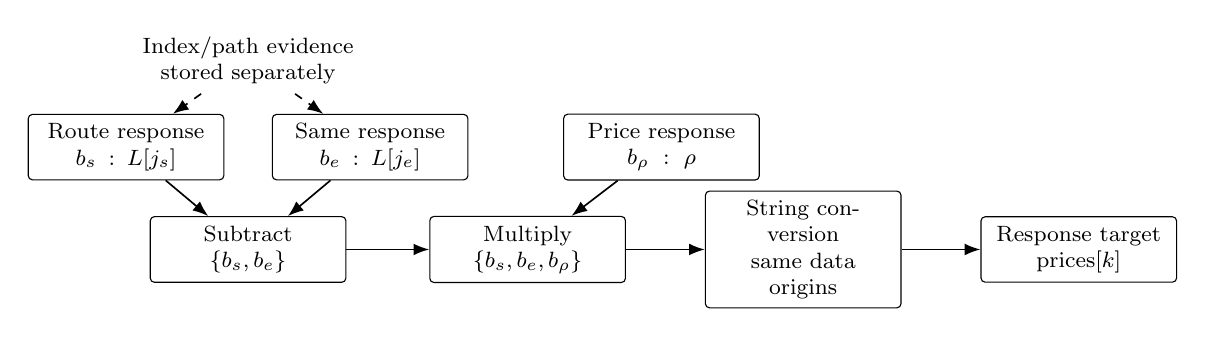
\begin{tikzpicture}[
    x=1cm,y=1cm,
    box/.style={draw,rounded corners=1.5pt,align=center,
        minimum height=0.72cm,text width=2.25cm,font=\footnotesize},
    arr/.style={-{Latex[length=2mm]},semithick},
    note/.style={align=center,font=\footnotesize}
]
\node[box] (start) at (0.9,0) {Route response\\$b_s: L[j_s]$};
\node[box] (end) at (4.0,0) {Same response\\$b_e: L[j_e]$};
\node[box] (rate) at (7.7,0) {Price response\\$b_\rho:\rho$};
\node[box] (diff) at (2.45,-1.3) {Subtract\\$\{b_s,b_e\}$};
\node[box] (mul) at (6.0,-1.3) {Multiply\\$\{b_s,b_e,b_\rho\}$};
\node[box] (render) at (9.5,-1.3) {String conversion\\same data origins};
\node[box] (target) at (13.0,-1.3) {Response target\\$\mathrm{prices}[k]$};
\node[note] (selection) at (2.45,1.1) {Index/path evidence\\stored separately};
\draw[arr] (start) -- (diff);
\draw[arr] (end) -- (diff);
\draw[arr] (diff) -- (mul);
\draw[arr] (rate) -- (mul);
\draw[arr] (mul) -- (render);
\draw[arr] (render) -- (target);
\draw[arr,dashed] (selection) -- (start);
\draw[arr,dashed] (selection) -- (end);
\end{tikzpicture}
\caption{Dependency propagation for the price example. Solid arrows show the
forward propagation of data origins; the stored query graph follows the
corresponding dependencies backward. Dashed arrows identify selection evidence.
Each source also retains its concrete message, object/member, and observation
coordinates. Equal numerical values do not merge the source occurrences.}
\label{fig:price-provenance}
\end{figure*}

\subsection{Cross-Service Graph and Response Binding}
\label{sec:method-graph}

Local reconstruction results, object-field forwarding, and communication
links are inserted into one dependency graph. Edges point from a result to
the instances it depends on. W3C trace context supplies communication
context; concrete RPC span/message identity, request or response direction,
and JSON pointer distinguish fields within it. Different messages in one
trace are not merged by trace ID.

A communication edge requires a unique compatible sending and receiving
field for that message and direction. Observed values are checked for
consistency only after this identity-based match. The receiving field is
connected to local computation through actual decoding, object, field,
version, and invocation evidence. Same-process forwarding similarly requires
a uniquely justified provider; it does not choose the latest equal value.

Finally, the serialized response target is linked to the reconstructed
provider at its actual root return coordinate. Let
$\mathcal{S}_B(E)$ be the source occurrences admitted by boundary $B$ in
capture $E$. For a successfully verified target $x$, the answer is
\begin{equation}
    \mathcal{P}_Q(x)=
    \{b\in\mathcal{S}_B(E)\mid x\leadsto b\}.
    \label{eq:answer}
\end{equation}
This set is reported as known only when the necessary reconstruction and
binding obligations have been discharged. A known constant can terminate
with an empty set. An unexplained leaf cannot.
The graph retains evidence coordinates and paths so that an answer can be
inspected back to its source observations.

\subsection{Guarded Observation Reduction}
\label{sec:method-reduction}

Full and selective modes use the same reconstruction semantics and required
validation. Full is bounded by the classes and methods admitted to the
task; it is not a trace of every JVM instruction. Shared implementation
cleanup is applied to both modes before attributing changes to query
specialization.

The current reductions have three distinct scopes. First, selective response
projection persists only the bound target response fields, while the
collector still obtains and checks the complete declared before/after
projections. It primarily reduces persisted fields and graph work rather
than all temporary field observations.

Second, within a declared read-return source call, selected simple
argument-assignment constructors can omit scalar write values outside the
conservative field obligations. Their bytecode, class hashes, source-call
extent, omission counts, and write-version maintenance are checked. This
does not permit a general constructor or source call to be skipped.

Third, ordinary writes in interpreted application Frames or bytecode-checked
setters can use a version-only record. Define
\begin{equation}
    R_Q=\{t\}\cup R_{\mathrm{field}}\cup
        R_{\mathrm{getter}}\cup R_{\mathrm{projection}},
    \label{eq:value-obligations}
\end{equation}
where the sets include \emph{all} planned application field reads, verified
getter reads, and constructor input projections. Only a supported scalar
field outside $R_Q$ is a candidate. The runtime checks the exact receiver
class and the actual rooted Frame or uniquely matched setter call.
The record retains owner, field, version, and site; the offline checker
verifies scope and version continuity. The omitted value is represented
as unknown if encountered, never recovered as a source from an output
snapshot. Reference-bearing effects, arguments, returns, branches,
containers, exceptions, and required snapshots remain observed.

These rules reduce selected value observations under explicit conditions.
They do not constitute a complete interprocedural slice, a minimum
observation plan, or permission to remove calls whose return values appear
unused.

\subsection{Worked Example and Answer States}
\label{sec:method-example}

Consider an original ticket-price computation,
\begin{equation}
    p=\operatorname{string}\big((L[j_e]-L[j_s])\times\rho\big),
    \label{eq:price}
\end{equation}
where $L$ is a distance list returned by one service and $\rho$ is a rate
returned by another. This expression explains the example; it is not
embedded as a business rule in the reconstruction engine.
The planner follows the target Map write through supported string
construction, arithmetic, indexed reads, and getters.

At runtime, the evidence identifies the actual list, selected indices,
rate field, RPCs, and target write. Offline reconstruction first obtains
the dependencies of the selected elements, then propagates them through
subtraction, multiplication, rendering, and the Map update, as illustrated
in Fig.~\ref{fig:price-provenance}. Even if two distance elements or two rate
fields have equal values, their concrete coordinates remain distinct.
The index and branch origins remain selection evidence. If the observed
handler writes a supported fixed fallback price, its data-source set is
known and empty.



The final result has one of the following states. A \emph{known} answer has a
verified source set, possibly empty. \texttt{unknown} means that necessary
semantics or effects remain unresolved despite otherwise usable evidence.
\texttt{analysis\_limited} means that a supported analysis budget or a required
interpreter capability is exceeded. \texttt{evidence\_invalid} denotes missing,
contradictory, or unclosed necessary evidence. \texttt{N/A} denotes a business
execution that produces no target; a null field actually present in the
response is still a target. A planning rejection is reported before runtime
and is not converted into a runtime unknown or N/A.

The current implementation is limited to its supported JVM instructions,
types, implementations, and reviewed contracts. General reflection/native
writes, arbitrary serialization, unrestricted framework callbacks, and
shared concurrent mutation are outside its guarantee. These limits qualify
which executions can be answered; they do not authorize guessing origins
from field names, output values, or expected test answers.


% Uncomment these after adding citations with \cite{...} in the text.
% \bibliographystyle{IEEEtran}
% \bibliography{reference}










\end{document}
